
\chapter{Binding simulation to GUIs (back annotation)}

Combining physical simulation and sensor network simulation allows to verify
the accurracy of the sensing process in relation with the physical process.
In most of the cases, the two activities are independent, but there are known situations
where a control loop exist.

This chapter will shortly discuss preliminary works where geographic data are
extracted (see chapter \ref{sec:chapter5}), analyzed, and processed to simulate the
the physical process:
\begin{enumerate}
\item loop between graphical planning, simulation synthesis, and graphic interfface control from simulation,
\item case of a mobile moving inside a set of sensors,
\item case of cellular automata representing physical process.
\end{enumerate}


In these situations the physical process spread over 2D or 3D spaces, that are
divided into a number of adjacent cells. One solution to keep track of evolutions 
is to use massive parallelism with a good computation candidate being cellular automata.


\section{Binding  simulator to the map browser}
Figure
\ref{fig:netSimul} shows a view on a map interface connected to an Occam simulation. 
This is a view of the Santander network retrieved in real time from {\tt http://smartsantander.eu},
with the sound network selected for display. Communication links are initially shown as red line,
but to demonstrate the simpulation effect, we switch to the green color for each node sending
a message. 

It is noticeable that the small networlk at the bottom left is finished, while le big network 
is still revealing information.


\begin{figure}[hbtp]
\begin{center}
\leavevmode 
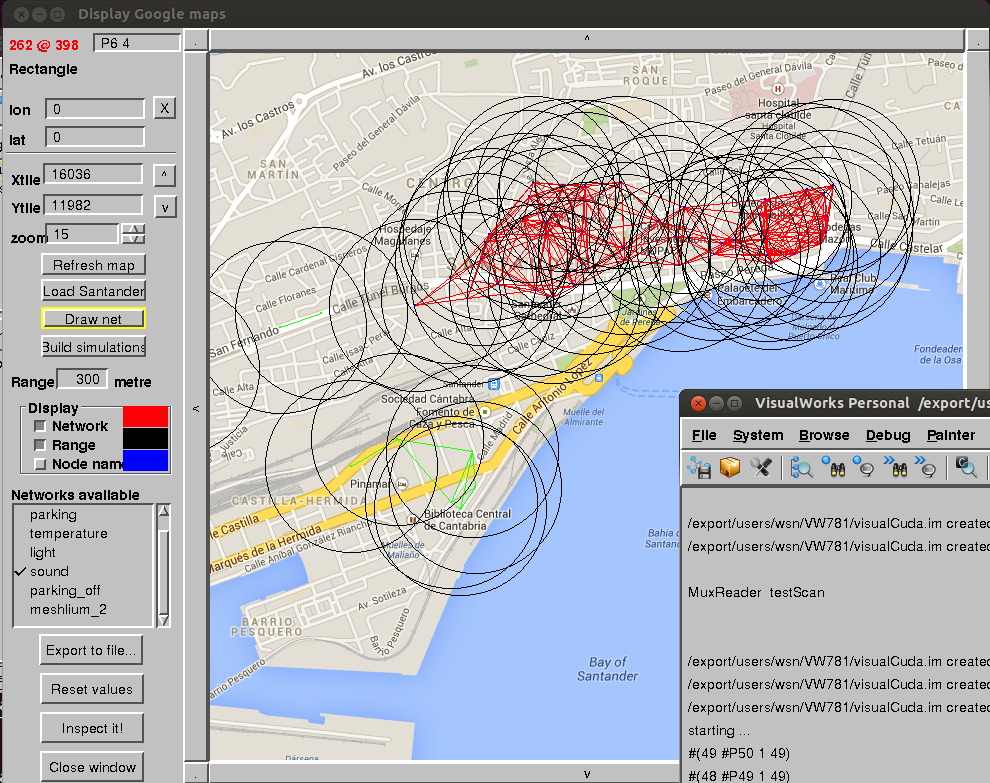
\includegraphics[width=12cm] {netSimul.png}
\caption{Feed back from concurrent simulation to Map Browser interface}
\label{fig:netSimul}
\end{center}
\end{figure}
 

This section will explain how the simulation, and even real messages from real sensors
can interact with the graphic view. Figure \ref{fig:mux4-st} presents the system organization, with
messages multiplexed to an Occam relay for an external process running Smalltalk.
In the Smalltalk image, messages are decoded and actions are taken to display visually
changes from simulation.

\begin{figure}[hbtp]
\begin{center} 
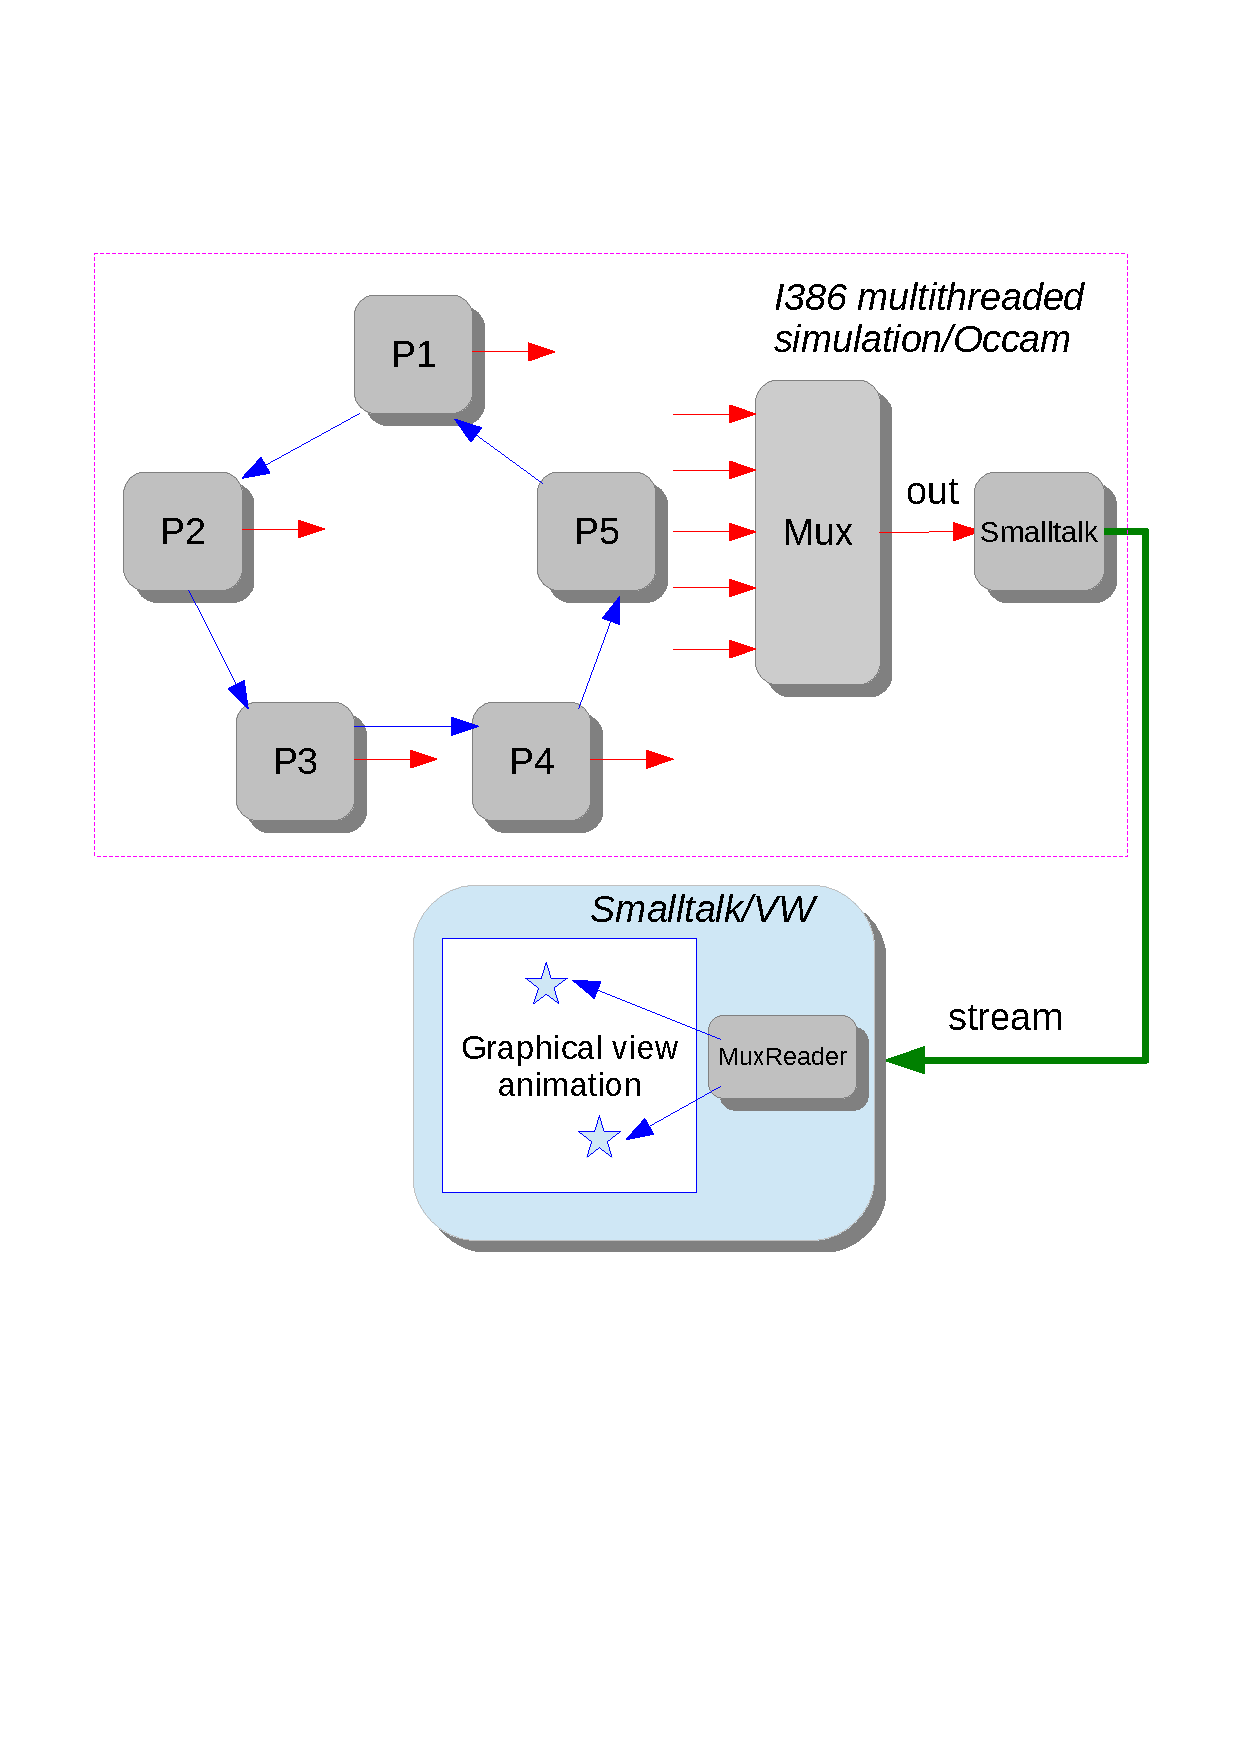
\includegraphics[width=10cm] {mux4-st.pdf}
\caption{System organization between simulator and graphical interface}
\label{fig:mux4-st}
\end{center}
\end{figure}
 

\subsection{Calling back the GUI}

The architecture description code source need support from an Occam mechanism allowing 
to fork external processes. The setup below will do, coupling a byte channel
to the i/o stream of this process.

\begin{lstlisting}
  PROC Smalltalk(   CHAN OF BYTE in , out , err )

    VAL [2][] BYTE Prog IS [ "/usr/local/vw7.8.1nc/bin/linux86/visual", "./visualnc.im" ]:
    VAL []BYTE arg IS  "./visualCuda.im":
    [2][100] BYTE Prog2 :
    [1]ENVIRONMENT envArray:
    INT result:
    SEQ
      -- nettoyer le tableau
      SEQ i=0 FOR 100
        SEQ
          Prog2[1][i] := (BYTE 0)
          Prog2[0][i] := (BYTE 0)
      -- copier la chaine de commande
      SEQ i=0 FOR SIZE Prog[0]
        Prog2[0][i] := Prog[0][i]
      -- copier la chaine argument
      SEQ i=0 FOR SIZE arg
        Prog2[1][i] := arg[i]
      -- configurer l'environnement
      proc.setenv (envArray[0], "VISUALWORKS" , "/usr/local/vw7.8.1nc")
      -- demarrer smalltalk
      out.string(Prog2[0],0,out)
      out ! ' '
      out.string(Prog2[1],0,out)
      out ! '*n'
      proc.wrapper(envArray, Prog2,  in , out , err, result)
  :
\end{lstlisting}


Inside the parallel construct, we now need to start a process that will fork a 
Visualworks image outside. The MuxToST channel will send information from
the Occam simulator multiplexer to the external Smalltalk GUI.
\begin{lstlisting} 
 [MaxNodes]CHAN OF BYTE toMux:
  CHAN OF BYTE MuxToST:
  PAR
    Smalltalk(MuxToST,stdout,stderr)
    Mux(toMux,MuxToST)
    Node(P1.in, P1.out,0, toMux [0])
    Node(P2.in, P2.out,1, toMux [1])
    Node(P3.in, P3.out,2, toMux [2])
....
\end{lstlisting}

\subsection{Passing contextual information to the simulator}.


For each process generated from NetGen, there is an entry in a varaible array.
The code below shows part of this array, where the data is simply the name 
of each process, as it appears in the network specification.

This name is a minimum information to advertise a GUI or tracer about the identity 
of an emitting process. 

\begin{lstlisting} 
VAL [51][3]BYTE NetProcess IS [   "P1 ", -- id: 1
  "P2 ", -- id: 2
  "P3 ", -- id: 3
  "P4 ", -- id: 4
  "P5 ", -- id: 5
  "P6 ", -- id: 6
  "P7 ", -- id: 7
  "P8 ", -- id: 8
  "P9 ", -- id: 9
  "P10", -- id: 10
....
]:
 \end{lstlisting}

The Mux relays information by sending the index of the channel, then copying the entire line to the
output.
 

\begin{lstlisting}
PROC Mux([]CHAN OF BYTE muxTab, CHAN OF BYTE out)
  BYTE c: 
  INT t:
  INT t64: 
  SEQ i=0 FOR ( MaxNodes)
    ALT i=0 FOR SIZE muxTab
      muxTab[i] ? c
        SEQ 
          out.number(i,4,out) 
          out !'*t'
          out ! c
          WHILE c <> '*n'
            SEQ
              muxTab[i] ? c
              out ! c
:
 \end{lstlisting}
\subsection {Demuxing in Smalltalk }

Lot of things can occur there by using Obectt oriented facilities for sensor attributes. In this demonstrator, 
we just decode lines sent from Smalltalk, select the sensor, displays its name, change colour all around,
an place the mouse over its location.

A class MuxReader has been developped for this, and the system code testScan  for decodint on the stream is showne below:
\lstinputlisting{MuxReaderclass-testScan.st}



